\documentclass[journal=jctcce,manuscript=suppinfo]{achemso}
% Supporting Information of the FastCREST paper. Build: pdflatex si; pdflatex si.
\usepackage[T1]{fontenc}
\renewcommand{\rmdefault}{ptm}
\renewcommand{\sfdefault}{lmss}
\renewcommand{\ttdefault}{lmtt}
\hyphenation{CREGEN FastCREST}
\usepackage{booktabs}
\usepackage{array}
\usepackage{amsmath}
\usepackage{url}
\usepackage{graphicx}

\newcommand{\Eh}{\ensuremath{E_\mathrm{h}}}
\newcommand{\quickflag}{\texttt{-{}-quick}}
\newcolumntype{L}[1]{>{\raggedright\arraybackslash}p{#1}}
\setlength{\emergencystretch}{2em}
\renewcommand{\thetable}{S\arabic{table}}
\renewcommand{\thefigure}{S\arabic{figure}}
\renewcommand{\thesection}{S\arabic{section}}

\title{FastCREST: GPU-Accelerated CREST Conformer Searches with Unchanged Energies and Gradients}

\author{Supantha Dey}
\affiliation{Department of Chemical and Biological Engineering, Iowa State University, Ames, Iowa 50011, United States}
\alsoaffiliation{Interdepartmental Genetics and Genomics Program, Iowa State University, Ames, Iowa 50011, United States}
\author{Nilusha Kariyawasam}
\affiliation{Department of Chemical and Biological Engineering, Iowa State University, Ames, Iowa 50011, United States}
\author{Ratul Chowdhury}
\email{ratul@iastate.edu}
\affiliation{Department of Chemical and Biological Engineering, Iowa State University, Ames, Iowa 50011, United States}

\begin{document}

\section{Search Settings, Software and Hardware}
\label{si:settings}

All iMTD-GC searches of the test system (274 atoms, charge $+4$, closed shell) started from the same structure and used
GFN2-xTB with ALPB water and \quickflag. FastCREST and conventional CREST searches were started with
\texttt{crest -{}-input search.toml -{}-newversion -{}-gfn2 -{}-chrg 4 -{}-uhf 0 -{}-alpb water -{}-quick -{}-ewin 5
-{}-noreftopo -T 32}; the input file sets the run type (\texttt{imtd-gc}), the calculation level and, for FastCREST,
\texttt{tblite\_solver = "cuda"}. The CREST 3.0.2 search used the equivalent command line of the release. In its command,
\quickflag{} followed \texttt{-{}-ewin 10} and reset the energy window to 5~kcal/mol, so the effective settings of all
searches are the same (Table~\ref{tab:si-settings}), except for the optimizer cycle limit (Section~\ref{si:cap}).

The CREST 3.0.2 release is the conda-forge build, which bundles a fork of tblite 0.3.0. FastCREST and conventional
CREST were built from CREST commit cfdc301f with tblite 0.5.0, gfortran 11.5 (\texttt{-O3}, no \texttt{-march}, so no
fused multiply--add instructions), OpenBLAS 0.3.27 and CUDA 12.4.1. Of the 200 files under \texttt{src/}, 151 are
identical in the two CREST trees, including the MD and MTD code, CREGEN and every optimizer file except the one with the
cycle limit.

All jobs ran on the Nova cluster of Iowa State University under Slurm. GPU nodes held A100 (40 and 80~GB), H200, V100,
L40S or RTX PRO 6000 GPUs, with AMD EPYC 7413, 7502, 7513, 7543 or 9645, AMD Zen~5 or Intel Xeon hosts. CPU-only searches
ran on EPYC 7502, Zen~4 (EPYC 9654) and Zen~5 (EPYC 9645) nodes; the optimizations run as Slurm array jobs went to
whichever CPU nodes the scheduler assigned.

\begin{table}[tbp]
\caption{Effective Search Settings of the iMTD-GC Searches of the Test System}
\label{tab:si-settings}
\small
\begin{tabular}{@{}L{0.27\textwidth}L{0.68\textwidth}@{}}
\toprule
item & setting \\
\midrule
algorithm & iMTD-GC, \quickflag \\
MTD & 6 trajectories per iteration, 250~ps each at 300~K; RMSD bias with push strengths 0.548 and 0.274 and widths $\alpha$ = 1.2, 0.6 and 0.3~bohr$^{-2}$; bias structures stored every 1~ps \\
integration & leap-frog, 5~fs time step, hydrogen mass 2~u, Berendsen thermostat (500~fs), snapshots every 100~fs \\
bond constraints & SHAKE on bonds with GFN0 Wiberg bond order $>0.5$ and length within $1.2(r_i+r_j)$; metal--ligand bonds never constrained (272 constraints) \\
MD stage & lowest one or two conformers, at 400 and 500~K, 125~ps each \\
optimizations & MTD snapshots crude, then regular; MD snapshots regular; genetic crossing crude, then regular; final ensemble tight \\
convergence (energy, gradient) & crude $5\times10^{-4}$~\Eh, $1\times10^{-2}$~\Eh~bohr$^{-1}$; regular $5\times10^{-6}$, $1\times10^{-3}$; tight $1\times10^{-6}$, $8\times10^{-4}$ \\
optimizer & ANCOPT; cycle limit one, three or five cycles per atom for crude, regular and tight thresholds, at least 200 (the CREST 3.0.2 search: 200, which the release can exceed by up to 39); \texttt{hlow} 0.005; 20 micro-iterations \\
CREGEN & energy window 5~kcal/mol (twice that at the crude level); RMSD 0.125~\AA; energy 0.05~kcal/mol; rotational constants 1\%; topology check on \\
genetic crossing & at most 2,500 structures \\
SCC & energy $1\times10^{-6}$~\Eh, density $2\times10^{-5}$ \\
\bottomrule
\end{tabular}
\end{table}

\section{Tests of the Computation}
\label{si:tests}

\paragraph{Configurations.} The tests compare nine configurations: the CREST 3.0.2 release; conventional CREST with the
command-line input and with the input file; FastCREST with the CPU solver, alone and with the warm-started Jacobi
eigensolver switched on; and FastCREST on the GPU, alone, with the Jacobi eigensolver, with the GPU-resident SCC, and
with both opt-in settings. Every GPU calculation had to show GPU use (an open CUDA session and the three-body term on
the GPU without a CPU fallback); all did.

\paragraph{Search setup.} Eight configurations replayed the search up to its first MTD. All made the same decisions as the
CREST 3.0.2 search: the same pre-optimized structure (energies of its first and last optimization steps $-415.2625315087$
and $-415.2625672259$~\Eh, the same to $1\times10^{-10}$~\Eh), flexibility measure 0.391, six MTD trajectories of
250~ps with the same bias settings, no failed trial MTD, 274 bonds with Wiberg bond order above 0.5 and 272 SHAKE
constraints.

\paragraph{Single points.} Energies and gradients were computed for 306 structures: the two input geometries, the 135
final conformers and 50 MD snapshots of the CREST 3.0.2 search, two steps of its first optimization, and 50 MD-stage
inputs and 67 conformers of a FastCREST search. The criterion was $|\Delta E| \le 10^{-8}$~\Eh{} and a largest gradient
component difference $\le 10^{-6}$~\Eh~bohr$^{-1}$; every structure met it in every comparison (Table~\ref{tab:si-sp}).
Our builds without the GPU gave bitwise identical results; the $10^{-10}$~\Eh{} between them and the release comes from
the different builds (tblite version, compiler and flags). The apo peptide and the Co, Cu and Ni complexes of a related peptide (241 or 242 atoms; the complexes open shell with one or two unpaired electrons) agreed as well: over ten structures each,
the release, FastCREST on the CPU and FastCREST on the GPU agreed within $1.1\times10^{-10}$~\Eh{} and
$7.4\times10^{-11}$~\Eh~bohr$^{-1}$.

\begin{table}[tbp]
\caption{Single Points of 306 Structures}
\label{tab:si-sp}
\small
\begin{tabular}{@{}L{0.46\textwidth}rrr@{}}
\toprule
 & bitwise & largest & largest $|\Delta g|$ \\
comparison & identical & $|\Delta E|$ (\Eh) & (\Eh~bohr$^{-1}$) \\
\midrule
conventional CREST vs the release & 0 & $1.01\times10^{-10}$ & $8.16\times10^{-11}$ \\
input file vs command line (conventional CREST) & 306 & 0 & 0 \\
FastCREST, CPU solver vs conventional CREST & 306 & 0 & 0 \\
FastCREST + Jacobi, CPU solver vs FastCREST, CPU solver & 306 & 0 & 0 \\
FastCREST, GPU vs the release & 0 & $1.01\times10^{-10}$ & $8.16\times10^{-11}$ \\
FastCREST + Jacobi, GPU vs the release & 0 & $1.00\times10^{-10}$ & $8.16\times10^{-11}$ \\
FastCREST + GPU-resident SCC vs the release & 0 & $1.00\times10^{-10}$ & $8.16\times10^{-11}$ \\
both opt-in settings vs the release & 0 & $1.00\times10^{-10}$ & $8.16\times10^{-11}$ \\
FastCREST, GPU vs CPU solver & 0 & $3.98\times10^{-13}$ & $4.0\times10^{-15}$ \\
FastCREST + Jacobi, GPU vs CPU solver & 0 & $3.41\times10^{-13}$ & $3.3\times10^{-14}$ \\
FastCREST + GPU-resident SCC vs CPU solver & 0 & $4.55\times10^{-13}$ & $4.0\times10^{-15}$ \\
both opt-in settings vs CPU solver & 0 & $4.55\times10^{-13}$ & $6.0\times10^{-15}$ \\
\bottomrule
\end{tabular}
\end{table}

\paragraph{Controlled MD.} Trajectories cannot be compared bit for bit, so we compared what matters for the search: how
often MD snapshots change their bonding topology, which decides how many structures CREGEN keeps. MD trajectories of
20~ps at 400 and 500~K started from four structures with the same initial velocities in every configuration (taken from
CREST restart files): seeds 1--3 for two structures and 1--8 for two structures of a later cycle, 44 trajectory pairs per
comparison (24 when only seeds 1--3 were run). Every tenth snapshot was optimized with the 200-cycle limit. For each pair
we took the difference $d$ in the fraction of snapshots whose topology differs from the input, before and after
optimization. A comparison passed if the 90\% confidence interval of the mean $d$ lay within $\pm0.15$ (two one-sided
tests; the margin was fixed before the runs). All 13 comparisons passed (Table~\ref{tab:si-md}). Paired trajectories
separated (all-atom RMSD above 0.5~\AA) after a median of 4.7 to 4.8~ps in every comparison with the release, and after
6.5~ps when the same build ran twice, so no configuration diverged early.

\begin{table}[tbp]
\caption{Controlled MD: 90\% Confidence Intervals of the Mean Difference in Topology-Change Fraction}
\label{tab:si-md}
\small
\begin{tabular}{@{}L{0.52\textwidth}rcc@{}}
\toprule
comparison & pairs & MD snapshots & after optimization \\
\midrule
conventional CREST run twice & 24 & $-0.024$ to $+0.017$ & $-0.084$ to $+0.041$ \\
conventional CREST vs the release & 44 & $-0.015$ to $+0.017$ & $-0.039$ to $+0.030$ \\
input file vs command line & 24 & $-0.005$ to $+0.034$ & $-0.030$ to $+0.110$ \\
FastCREST, CPU solver vs conventional CREST & 24 & $-0.043$ to $+0.005$ & $-0.137$ to $-0.007$ \\
FastCREST, GPU vs CPU solver & 24 & $-0.000$ to $+0.050$ & $+0.008$ to $+0.134$ \\
FastCREST, GPU vs conventional CREST & 44 & $-0.001$ to $+0.030$ & $+0.005$ to $+0.072$ \\
FastCREST, GPU vs the release & 44 & $-0.003$ to $+0.033$ & $-0.014$ to $+0.082$ \\
FastCREST + Jacobi vs FastCREST, GPU & 44 & $-0.033$ to $+0.010$ & $-0.076$ to $+0.025$ \\
FastCREST + Jacobi vs the release & 44 & $-0.020$ to $+0.026$ & $-0.048$ to $+0.064$ \\
FastCREST + GPU-resident SCC vs FastCREST, GPU & 44 & $-0.024$ to $+0.016$ & $-0.065$ to $+0.040$ \\
both opt-in settings vs FastCREST + Jacobi & 44 & $-0.021$ to $+0.021$ & $-0.059$ to $+0.040$ \\
FastCREST + GPU-resident SCC vs the release & 44 & $-0.005$ to $+0.027$ & $-0.029$ to $+0.072$ \\
both opt-in settings vs the release & 44 & $-0.013$ to $+0.020$ & $-0.044$ to $+0.042$ \\
\bottomrule
\end{tabular}
\end{table}

\paragraph{Optimizer cycle limit.}
\label{si:cap}
CREST commit 9908b42, between the 3.0.2 release and cfdc301f, stops an unconverged ANCOPT optimization exactly at its
cycle limit; the release lets it finish its last relaxation block, which at a limit of 200 cycles means up to 239. Unconverged optimizations are discarded, so the earlier stop can only remove structures. We optimized 100 MD snapshots of each of two sets at the regular level
(Table~\ref{tab:si-cap}). The earlier stop left 2 to 3 more of every 100 unconverged, more than the 1 per 100 we had set as acceptable; runs with a 240-cycle limit put an upper bound of 4 to 8 per 100 on the difference (Table~\ref{tab:si-cap}). Structures converged in both versions passed
or failed CREST's topology check alike, and their energies differed by at most $1.5\times10^{-3}$~\Eh, as optimizations
in different builds do. We kept the commit.

This test used a limit of 200 cycles in both versions, as CREST does in its searches. ANCOPT derives the limit from the
number of atoms when none is set (Table~\ref{tab:si-settings}), by the same rule as the optimizer of the xtb program,
which ran CREST's optimizations before version 3. In every CREST 3 version (3.0, 3.0.1, 3.0.2 and the current code),
however, the routine that writes the optimization settings to the output also sets the limit to 200 for the rest of the
search. FastCREST's version of that routine changes no setting, so each optimization keeps the size-dependent limit, and
structures that stay unconverged after 200 cycles can still converge. Every replicate search, FastCREST and
conventional CREST, used the size-dependent limit.

\begin{table}[tbp]
\caption{Optimizations Converged at a Limit of 200 Cycles, out of 100}
\label{tab:si-cap}
\small
\begin{tabular}{@{}L{0.42\textwidth}rrrr@{}}
\toprule
snapshots & release & our builds & difference & upper bound \\
\midrule
MD stage of the CREST 3.0.2 search, second cycle & 95 & 92 & 3 & 8 \\
MD stage of a FastCREST search, second cycle & 93 & 91 & 2 & 4 \\
\bottomrule
\end{tabular}
\end{table}

\section{Replicate Searches}
\label{si:replicates}

The comparison was fixed before any group summary was computed. The compared quantity is the lowest energy after the crude
optimization of the first MTD iteration (14,994 snapshots, the same CPU optimizer in every search), taken from every
search that reached that point, finished or not, because searches with fewer cycles finish first. The groups are FastCREST on
the GPU and conventional CREST, that is, our builds run on CPUs only, whose single points are bitwise identical to
those of CREST built without our patches. The statistic is the Hodges--Lehmann shift (FastCREST minus conventional CREST) with exact Mann--Whitney
confidence intervals. A difference is detected if the 95\% interval excludes zero; equivalence is shown if the 90\%
interval lies within $\pm2$~kcal/mol (under half the 5~kcal/mol energy window); otherwise the result is inconclusive.

Sixteen of 40 FastCREST searches and 17 of 18 conventional CREST searches reached that point
(Table~\ref{tab:si-searches}). Most of the other FastCREST searches stopped within seconds on one GPU with a memory error
and were not restarted. The 16 that reached it ran their first iteration on 9 L40S, 3 V100, 3 A100 and 1 H200 GPU; 13 of
them, but 7 of the 17 conventional searches, resumed from checkpoints before that point. The shift was $+4.09$~kcal/mol
(95\% interval $-4.94$ to $+11.75$, achieved level 0.951; 90\% interval $-3.58$ to $+10.13$; two-sided $p = 0.35$): no
difference detected and equivalence not shown. With only the four FastCREST searches on A100 or H200 GPUs the shift
was $+3.12$ ($-14.50$ to $+19.80$), and against only the nine conventional searches with FastCREST's own build on the
CPU, $+2.75$ ($-6.44$ to $+13.89$). The final energies of the finished searches (10 FastCREST, 15 conventional) gave a shift of $-2.70$~kcal/mol
(95\% interval $-11.27$ to $+6.54$), a comparison chosen after the data were seen.

\begin{table}[tbp]
\caption{Replicate Searches of the Test System. Energies in kcal/mol Relative to the Lowest Final Conformer of These Searches (Conventional 7, $-415.48139$~\Eh)}
\label{tab:si-searches}
\small
\begin{tabular}{@{}llrrrr@{}}
\toprule
search & GPU & first MTD iteration & final & conformers & new cycles \\
\midrule
conventional 1 & CPU & $+$13.1 & $+$16.7 & 19 & 1 \\
conventional 2 & CPU & $+$16.8 & $+$16.4 & 8 & 1 \\
conventional 3 & CPU & $+$21.1 & $+$25.2 & 3 & 2 \\
conventional 4 & CPU & $+$22.3 & not finished &  &  \\
conventional 5 & CPU & $+$24.5 & $+$4.5 & 7 & 3 \\
conventional 6 & CPU & $+$26.4 & not finished &  &  \\
conventional 7 & CPU & $+$29.4 & $+$0.0 & 3 & 1 \\
conventional 8 & CPU & $+$29.5 & $+$7.6 & 2 & 2 \\
conventional 9 & CPU & $+$32.1 & $+$20.2 & 12 & 1 \\
conventional 10 & CPU & $+$32.7 & $+$16.7 & 1 & 1 \\
conventional 11 & CPU & $+$34.0 & $+$15.5 & 12 & 2 \\
conventional 12 & CPU & $+$34.7 & $+$11.7 & 34 & 2 \\
conventional 13 & CPU & $+$35.0 & not finished &  &  \\
conventional 14 & CPU & $+$38.0 & $+$124.7 & 11 & 0 \\
conventional 15 & CPU & $+$41.1 & $+$116.0 & 10 & 0 \\
conventional 16 & CPU & $+$53.3 & $+$3.7 & 82 & 2 \\
conventional 17 & CPU & $+$54.7 & $+$20.0 & 1 & 3 \\
conventional 18 & CPU & -- & $+$12.1 & 9 & 1 \\
FastCREST 1 & H200 & $+$17.2 & not finished &  &  \\
FastCREST 2 & L40S & $+$18.2 & $+$3.6 & 22 & 2 \\
FastCREST 3 & L40S & $+$22.5 & not finished &  &  \\
FastCREST 4 & L40S & $+$23.2 & $+$1.9 & 51 & 1 \\
FastCREST 5 & A100 & $+$26.6 & $+$8.7 & 3 & 2 \\
FastCREST 6 & L40S & $+$31.4 & $+$32.8 & 40 & 2 \\
FastCREST 7 & L40S & $+$34.0 & not finished &  &  \\
FastCREST 8 & L40S & $+$34.7 & $+$14.1 & 1 & 2 \\
FastCREST 9 & L40S & $+$36.2 & $+$30.0 & 5 & 1 \\
FastCREST 10 & V100 & $+$37.1 & not finished &  &  \\
FastCREST 11 & V100 & $+$40.9 & not finished &  &  \\
FastCREST 12 & A100 & $+$42.1 & $+$9.2 & 20 & 3 \\
FastCREST 13 & V100 & $+$42.2 & not finished &  &  \\
FastCREST 14 & L40S & $+$47.7 & $+$8.9 & 173 & 1 \\
FastCREST 15 & A100 & $+$49.5 & $+$14.2 & 103 & 2 \\
FastCREST 16 & L40S & $+$50.8 & $+$17.1 & 19 & 1 \\
FastCREST + Jacobi & A100 & $+$37.9 & $+$33.1 & 10 & 2 \\
\bottomrule
\end{tabular}


\smallskip
\begin{minipage}{\textwidth}\raggedright\footnotesize
First MTD iteration: lowest energy after its crude optimization (the quantity compared). Final: lowest energy of
the final ensemble. New cycles: cycles started after the MD stage or genetic crossing found a lower conformer. GPU: the
GPU of the first iteration; conventional CREST ran on CPUs. Conventional 18 has no first-iteration value: its first iteration was
replayed from a checkpoint and its crude optimization was not kept.
\end{minipage}
\end{table}

\section{Time per MTD Step on Other Hardware}
\label{si:hardware}

Table~\ref{tab:si-hardware} lists the time per MTD step of the test system measured in searches and benchmarks on other
nodes. The host CPU matters as much as the GPU, because most of each step is still CPU work.

\begin{table}[tbp]
\caption{Time per MTD Step of the Test System on Different Hardware}
\label{tab:si-hardware}
\small
\begin{tabular}{@{}L{0.50\textwidth}rrr@{}}
\toprule
 & & & times faster than \\
code and hardware & threads & s per step & the CREST 3.0.2 search \\
\midrule
CREST 3.0.2 search, node not recorded & 32 & 2.8 & 1.0$\times$ \\
conventional CREST with the thread settings, EPYC 7502 & 32 & 1.43--1.51 & 1.9$\times$ \\
same, whole EPYC 7502 node & 64 & 1.35--1.37 & 2.1$\times$ \\
FastCREST without GPU, EPYC 7502 & 64 & 1.26--1.27 & 2.2$\times$ \\
FastCREST without GPU, Zen~4 (shared node) & 64 & 0.93 & 3.0$\times$ \\
FastCREST without GPU, Zen~5 (shared node) & 64 & 0.74 & 3.8$\times$ \\
FastCREST, V100 and an older Intel Xeon\textsuperscript{\emph{a}} & 8 & 1.86 & 1.5$\times$ \\
FastCREST, RTX PRO 6000 and EPYC 9645\textsuperscript{\emph{a}} & 32 & 0.68 & 4.1$\times$ \\
FastCREST, A100 and EPYC 7543 & 32 & 0.46--0.49 & 5.7--6.0$\times$ \\
FastCREST, H200 and Zen~5 & 32 & 0.39 & 7.1$\times$ \\
\bottomrule
\end{tabular}

\smallskip
\begin{minipage}{\textwidth}\raggedright\footnotesize
Ranges: two runs or two nodes. The hosts differ between rows, so the factors combine the code and the hardware; on the
same A100 nodes FastCREST was 5.5 times faster than conventional CREST (main text, Figure~2b).
\textsuperscript{\emph{a}}No GPU code for this architecture in the build: the three-body term ran on the CPU. V100: one
partial trajectory.
\end{minipage}
\end{table}

\section{Other CREST Run Types}
\label{si:modes}

CREST's other run types use the same trajectory and optimization code, so FastCREST runs them as well. We compared each with CREST built from the same commit without our patches, which stops optimizations after 200 cycles (Section~\ref{si:cap}; Table~\ref{tab:si-modes}). Protonation, deprotonation and tautomer
searches have no MD and gave the same structures and energies. The NCI-MTD and entropy runs are adaptive and scatter
from run to run in both codes; where runs were repeated, their results agree within that scatter. The taxol entropy runs and the NCI-MTD search of the test system ran once per code. One NCI-MTD search of the test system was also
run with FastCREST and with the CREST 3.0.2 release (last NCI-MTD row). With the wall potential of NCI-MTD, FastCREST
runs the optimizations in the main job rather than as array jobs, so its gain is smaller than in iMTD-GC searches.

\begin{table}[tbp]
\caption{Other Run Types with FastCREST and Conventional CREST}
\label{tab:si-modes}
\small
\begin{tabular}{@{}L{0.17\textwidth}L{0.25\textwidth}L{0.52\textwidth}@{}}
\toprule
run type & molecule & result \\
\midrule
protonation, deprotonation, tautomers & uracil, caffeine, guanine (gas phase) & same structures and energies in every run (fastest mode: largest $|\Delta E|$ $6.4\times10^{-6}$~\Eh) \\
protonation & Ga(III)--peptide (132 atoms, $+3$, ALPB water) & lowest protomer the same within $2\times10^{-6}$~\Eh{} in all runs; the number of structures kept varies from run to run in conventional CREST itself (53, 69 and 60) as in FastCREST (74 and 58) \\
NCI-MTD & water trimer (gas phase) & same lowest energy ($-15.235025$~\Eh) in all nine runs \\
NCI-MTD & Ga(III)--peptide (132 atoms, ALPB water, \quickflag) & lowest energies of six runs within 1.8~kcal/mol; conventional CREST 59.6 and 217.7~min, FastCREST 18.1 and 29.0~min (3.3 and 7.5 times faster in the two pairs of runs, different nodes), fastest mode 14.6 and 16.0~min \\
NCI-MTD & test system (ALPB water) & one search each from the same structure: CREST 3.0.2 release 93.7~h (32 threads, EPYC 7502 node), FastCREST 34.2~h (A100 GPU, EPYC 7513 host; 2.7 times faster, with three MTD iterations against two); lowest energies 5.0~kcal/mol apart (FastCREST higher); 1 conformer with FastCREST, 7 with the release \\
entropy & $n$-octane (gas phase) & conformational entropy 8.12~cal~mol$^{-1}$~K$^{-1}$ (FastCREST), 8.13 (fastest mode), 8.20, 8.20 and 8.32 (conventional CREST); for this 26-atom molecule FastCREST took 14.8~min and conventional CREST 7.3~min (2.0 times slower) \\
entropy & taxol (113 atoms, ALPB water, \quickflag) & conformational entropy 9.65 (conventional CREST, 63.3~h), 9.89 (FastCREST, 46.5~h, 1.4 times faster) and 9.37~cal~mol$^{-1}$~K$^{-1}$ (fastest mode, 21.6~h, 2.9 times faster); different nodes \\
\bottomrule
\end{tabular}
\end{table}

\section{CREST's New-Cycle Step and FastCREST's Opt-in Fixes}
\label{si:cycle}

When CREST's iMTD-GC search finds a lower conformer, two things in its code (CREST 3.0.2 and cfdc301f; the search
routine that the command line runs) do not do what the code intends. First, the routine that registers the new lowest
conformer deletes every \texttt{crest\_rotamers} file before the caller saves the newest of them for the next merge, so
when the MD stage or genetic crossing starts a new cycle, the ensemble found so far is lost and the next cycle merges
only its own MTD iterations. Second, the new lowest conformer is written to the file \texttt{coord} as the start of the
next MTD trajectories, but this routine never reads it again: every MTD trajectory starts from the input structure. CREGEN's
topology check, however, compares with \texttt{coord}.

Of the 26 finished replicate searches of the test system, 24 started at least one new cycle after the MD stage or genetic
crossing (41 new cycles in all), in conventional CREST and FastCREST alike (Table~\ref{tab:si-searches}); with the lower conformers
found inside MTD loops, the next MTD trajectories restarted from the input structure 60 times. Because both codes share
this behavior, it does not affect the comparison between them, but it explains why a final ensemble can lie far above
the lowest conformer seen during a search.

{\sloppy FastCREST 1.3.0 fixes both steps on request. With \texttt{CREST\_KEEP\_ENSEMBLE=1} the newest ensemble is copied before
it is deleted and joins every later merge; with \texttt{CREST\_RESTART\_FROM\_BEST=1} the next MTD trajectories start from
the new lowest conformer. With both unset, FastCREST computes what it did before: in a search forced into a second cycle,
the conformers and the search log were identical to the previous version, and single points were byte-identical. With
both set, the forced search restarted from the new lowest conformer, kept the earlier ensemble, and resumed normally when
killed at each of its 33 tracked steps.\par}

\section{Zn-Binding Test Peptides}
\label{si:metal}

Three 12-residue $\alpha$-helices with random sequences (no Cys or Pro, one His, at least one Asp or Glu) were built in
PyMOL: \mbox{DEGLAHSMAAFK} (p1), \mbox{GINGQALHAEYW} (p2) and \mbox{LKERTTEIHENI} (p3), with neutral termini, Asp and Glu deprotonated and
Lys and Arg protonated. A Zn$^{2+}$ ion was placed 2.05~\AA{} from the His NE2 (charge $+1$; 174 to 211 atoms). p1 was
also built with Asp and Glu protonated (low pH, charge $+3$). Each system was searched once with conventional CREST (the
3.0.2 release, 32 CPU cores), with FastCREST 1.2.0 and with FastCREST 1.3.0 with both opt-in fixes
(Section~\ref{si:cycle}); FastCREST ran as in the main text, on one A100 or H200 GPU. All searches used GFN2-xTB, ALPB
water, \quickflag{} and \texttt{-{}-noreftopo}; FastCREST used the size-dependent cycle limit
(Table~\ref{tab:si-settings}), conventional CREST the cap of 200 cycles. The Zn was left out of CREGEN's topology check
(\texttt{-{}-notopo} with its atom number), because the check counts metal--ligand contacts as bonds and removes every structure in which the Zn
changes partners: with the default check, a FastCREST search of p3 ended 119~kcal/mol above the lowest structure of
Table~\ref{tab:si-zn}, with the Zn still on the His.

In every search with the Zn left out of the topology check, the peptide wraps around the Zn (Figure~\ref{fig:si-zn},
Table~\ref{tab:si-zn}). The helix unwinds, the Zn becomes six-coordinate (seven-coordinate in one structure), its first
and last donor residues lie 5 to 9 positions apart, and the radius of gyration falls from 6.6--6.8~\AA{} to
5.4--6.0~\AA. At neutral pH the donors are the His, Asp and Glu carboxylates and backbone carbonyls, in p2 also the
N-terminal amine and the Asn3 side chain; in p3 the carboxylates take five or six sites and the His is released. At low
pH the His binds with four or five backbone carbonyl oxygens.

FastCREST 1.2.0 finished every system in 13 to 34~h (42 to 79~h with both fixes, which add cycles). Conventional CREST
finished only low-pH p1, in 97~h (FastCREST 7.3 times faster); its searches of p2 and p3 were not finished after 6~days
(FastCREST at least 10 and 4.2 times faster). In p1 the first optimization formed two bonds at the N-terminus that the
input lacks. CREGEN compares with the input and removed all or nearly all structures of the MTD trajectories, which start
from the optimized structure, so valid structures came from the MD stages; with the restart fix, the MTD trajectories of
later cycles started from a valid structure. The conventional search of p1 had finished two MTD iterations without a valid
structure when we stopped it after 53~h. The finished conventional search ended 9.1~kcal/mol above the lowest structure
it had found, through the new-cycle step of Section~\ref{si:cycle}. With both fixes, FastCREST gave the lowest final
structure of any search for p1, p2 and p3. Each system was searched once per code; run-to-run scatter
(Section~\ref{si:replicates}) was not measured for these systems.

Where both codes produced structures, they bind the Zn with mostly the same donors (Figure~\ref{fig:si-zn-overlap}).
Superposed on the Zn site, the lowest structures of the two codes lie 2.2 to 2.8~\AA{} apart (RMSD over the Zn, the
backbone of the binding residues and their donor groups) and share five or six donors; the two FastCREST searches of
each peptide differ from each other by 1.7 to 3.3~\AA{} on the same atoms. The chain ends differ more (C$\alpha$ RMSD
3.8 to 4.1~\AA).

\begin{figure}[tbp]
\centering
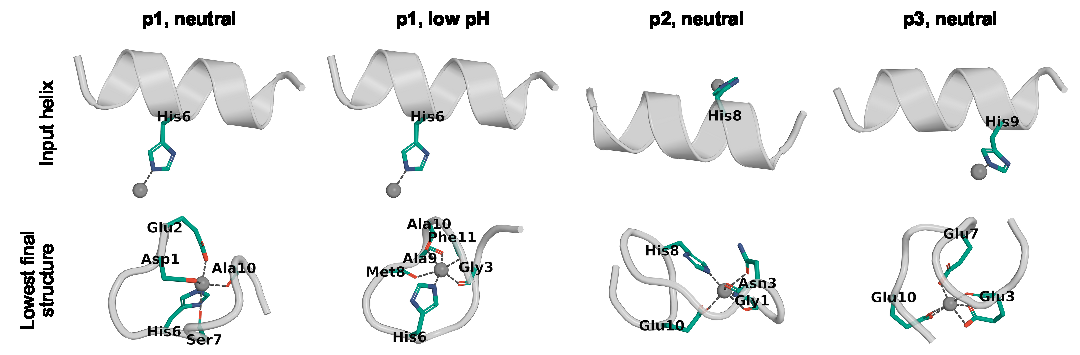
\includegraphics[width=\textwidth]{figures/si_zn_peptides.pdf}
\caption{Input helix (top) and lowest final structure (bottom; FastCREST with both fixes) of each peptide, all at the
same scale. Gray sphere: Zn; dashes: donors within 2.5~\AA; green sticks: the binding groups. Rendered with open-source
PyMOL.}
\label{fig:si-zn}
\end{figure}

\begin{figure}[tbp]
\centering
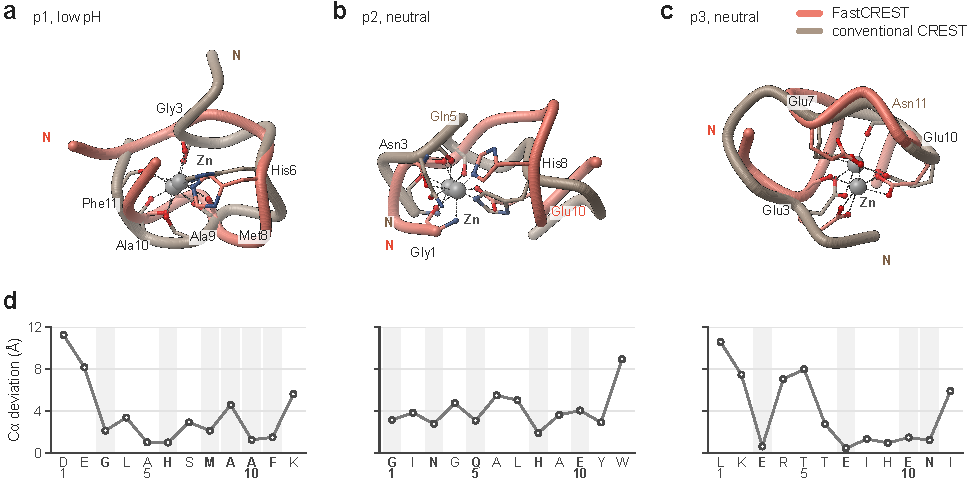
\includegraphics[width=\textwidth]{figures/si_zn_overlap.pdf}
\caption{Lowest structures found by FastCREST with both fixes (red) and by conventional CREST (brown) for (a) low-pH
p1, (b) p2 and (c) p3, superposed on the Zn site (the Zn, the backbone of the Zn-binding residues and their side-chain
donor groups). Dashes join the Zn (gray) to its donors; residue names in red or brown bind the Zn in only one
structure. (d) C$\alpha$ deviation per residue after this superposition; shaded residues bind the Zn in either
structure. Conventional CREST: for low-pH p1, the lowest structure its search found, which a new cycle dropped from its
final result; for p2 and p3, the lowest structure found before the 6-day limit. Neutral p1 is not shown, because
conventional CREST gave no structure.}
\label{fig:si-zn-overlap}
\end{figure}

\begin{table}[tbp]
\caption{Searches of the Zn-Binding Test Peptides. Energies in kcal/mol Relative to the Lowest Structure Found by Any
Search of That System}
\label{tab:si-zn}
\small
\setlength{\tabcolsep}{4pt}
\begin{tabular}{@{}L{0.10\textwidth}L{0.235\textwidth}rrL{0.37\textwidth}r@{}}
\toprule
system & search & time (h) & energy & Zn donors (CN) & $R_\mathrm{g}$ (\AA) \\
\midrule
p1 & FastCREST & 32.6 & $+2.5$ & His6; Glu2 (2 O); backbone O of Met8, Ala9, Ala10 (6) & 5.42 \\
 & FastCREST + both fixes & 41.8 & 0.0 & His6; Asp1 (2 O); Glu2; backbone O of Ser7, Ala10 (6) & 5.43 \\
 & conventional CREST\textsuperscript{\emph{a}} & 53 & & no valid structure & \\
p1, low pH & FastCREST & 13.3 & $+7.1$ & His6; backbone O of Gly3, Leu4, Ala9, Ala10, Phe11 (6) & 5.55 \\
 & FastCREST + both fixes & 43.6 & $+3.3$ & His6; backbone O of Gly3, Met8, Ala9, Ala10, Phe11 (6) & 5.50 \\
 & conventional CREST & 96.9 & $+9.1$ & His6; backbone O of Met8, Ala9, Ala10, Phe11; Met8 S (6) & 5.99 \\
 & \quad lowest found\textsuperscript{\emph{b}} & & 0.0 & His6; backbone O of Gly3, Met8, Ala9, Ala10, Phe11 (6) & 5.46 \\
p2 & FastCREST & 14.3 & $+2.8$ & His8; Glu10 (2 O); Asn3 OD1; backbone O of Gly1, Gln5 (6) & 5.72 \\
 & FastCREST + both fixes & 41.5 & 0.0 & His8; Glu10; Gly1 N and O; Asn3 O and OD1 (6) & 5.96 \\
 & conventional CREST\textsuperscript{\emph{c}} & $>$144 & $+1.6$ & His8; Gly1 N and O; Asn3 O and OD1; Gln5 O (6) & 5.79 \\
p3 & FastCREST & 34.4 & $+6.2$ & Glu3 (2 O); Glu7; Glu10 (2 O); Asn11 O (6) & 6.02 \\
 & FastCREST + both fixes & 79.1 & 0.0 & Glu3 (2 O and backbone O); Glu7; Glu10 (2 O) (6) & 5.62 \\
 & conventional CREST\textsuperscript{\emph{c}} & $>$144 & $+2.2$ & Glu3, Glu7, Glu10 (2 O each); Asn11 O (7) & 5.73 \\
\bottomrule
\end{tabular}

\smallskip
\begin{minipage}{\textwidth}\raggedright\footnotesize
FastCREST: version 1.2.0; with both fixes: version 1.3.0. Time: elapsed time of the main job, summed over the jobs the
search ran in. Energy, donors (within 2.5~\AA{} of Zn; CN, coordination number) and radius of gyration $R_\mathrm{g}$ of
the peptide heavy atoms: lowest final structure; $R_\mathrm{g}$ of the inputs: 6.68 (p1), 6.62 (p2) and 6.80~\AA{} (p3).
\textsuperscript{\emph{a}}Stopped by us after two MTD iterations. \textsuperscript{\emph{b}}Lowest structure the
conventional search found; a new cycle dropped it from the final result. \textsuperscript{\emph{c}}Not finished after
6~days: lowest structure found.
\end{minipage}
\end{table}

\section{A Second Ga(III)--Peptide Complex}
\label{si:ga2}

The peptide \mbox{MLTREQIEELSKLLE} differs from the test system in two residues (Leu13 and Glu15 instead of Lys). Its Ga(III)
complex has 264 atoms and charge $+1$ and is closed shell, with neutral termini, the four Glu deprotonated and Arg4 and
Lys12 protonated (pH~8). In the preoptimized helical input, Ga binds six oxygens (Table~\ref{tab:si-pep023}). The complex
was searched once with each code from this input, with GFN2-xTB, ALPB water, \quickflag{} and \texttt{-{}-noreftopo} as
for the test system (final energy window 5~kcal/mol): conventional CREST (CREST 3.0.2) on 32 threads of an AMD Zen~5
node, and FastCREST 1.1.1 on one A100 GPU with an AMD EPYC 7543 host, with its optimizations run as 1,583 Slurm array
tasks on other nodes (6,060 allocated CPU-hours).
The two codes also used different optimizer cycle limits (Section~\ref{si:cap}): 200 cycles in CREST 3.0.2, and 264, 792
and 1,320 cycles for crude, regular and tight thresholds in FastCREST. In the two MD stages, 3,013 of 5,061 and 3,220 of
5,028 optimizations converged in CREST 3.0.2, and all of them in FastCREST.
FastCREST took 58.4~h and conventional CREST 265.8~h, so FastCREST was 4.6 times faster, on different hardware and with
more work: it ran three cycles (six MTD iterations) and conventional CREST two (four). Per MTD iteration, FastCREST took
7.2~h and conventional CREST 35.2~h (4.9 times faster). No trajectory stopped early in either search.

Both searches ended near the input (Figure~\ref{fig:si-pep023}a--c). As in the test system, every structure kept the
Ga--O bonds of the input, and every conformer of both final ensembles kept the nine helical residues of the input and
lies within 1.5~\AA{} of it (C$\alpha$ RMSD). The two lowest final conformers coincide on the Ga site (RMSD 0.08~\AA) and
differ by 0.7~\AA{} over all C$\alpha$ atoms, mostly at Met1; FastCREST's lies 1.1~kcal/mol lower. The final ensembles
overlap: each of the 79 conventional CREST conformers lies within 1.1~\AA{} (C$\alpha$ RMSD) of one of the 48 FastCREST
conformers. Both searches had found lower structures that a new cycle then dropped (Section~\ref{si:cycle}). Conventional
CREST's lies 2.4~kcal/mol below FastCREST's lowest final conformer and only 0.2~\AA{} from it (C$\alpha$ RMSD).
FastCREST's, found in its second cycle, lies 30.7~kcal/mol below it with the same Ga--O bonds, but the helix has
unfolded into a compact structure (radius of gyration 6.7~\AA, input 7.5~\AA; Figure~\ref{fig:si-pep023}b, dashed).
FastCREST's final ensemble comes from its third cycle, whose trajectories started again from the input. With one search
per code, run-to-run scatter (Section~\ref{si:replicates}) was not measured for this complex.

\section{An Open-Shell Fe(II) Complex}
\label{si:fe}

The high-spin Fe(II) complex of the same peptide (264 atoms, charge 0, four unpaired electrons, with the protonation
states and neutral termini of Section~\ref{si:ga2}) was searched once with each code (an earlier FastCREST search, cut short by bugs fixed in versions 1.1.1 and 1.1.2, is not used), with the codes and settings of
Section~\ref{si:ga2}, from one preoptimized helical input in which Fe binds three oxygens. Conventional CREST took 242.3~h on 32 threads of an
Intel Skylake node, and FastCREST 7.3~h on one A100 GPU with an AMD EPYC 7513 host (63 array tasks, 222 CPU-hours). Both
searches finished normally, but most trajectories stopped early in both codes: 48 of 50 MTD and MD trajectories in
conventional CREST and all 20 in FastCREST, and the MTD iterations produced only 2 to 29\% of the snapshots of a complete
iteration. Neither search therefore sampled as intended. The two times are not comparable: conventional CREST ran four
cycles and FastCREST one, both with truncated trajectories.

The two searches ended in different structures (Figure~\ref{fig:si-pep023}d,e; Table~\ref{tab:si-pep023}). Conventional
CREST's lowest final conformer stayed close to the input (C$\alpha$ RMSD 1.3~\AA) and binds Fe through the three oxygens
of the input and a carboxylate oxygen of Glu5. FastCREST's is compact and binds Fe through five backbone carbonyl oxygens
and the side-chain oxygen of Gln6, with no carboxylate; it lies 85.5~kcal/mol lower. In its third cycle, conventional
CREST had found a structure 13.7~kcal/mol below FastCREST's lowest final conformer, also compact and without a
carboxylate donor, but a new cycle dropped it (Section~\ref{si:cycle}), and the final ensemble ended 99.2~kcal/mol above
it. Single points gave the same energies with CREST 3.0.2 and FastCREST for the final conformers of both searches
(within $9\times10^{-11}$~\Eh), so the energy differences come from different structures, not from different energies for the same structure. The
structures and energies are GFN2-xTB results that we did not validate further.

\begin{figure}[tbp]
\centering
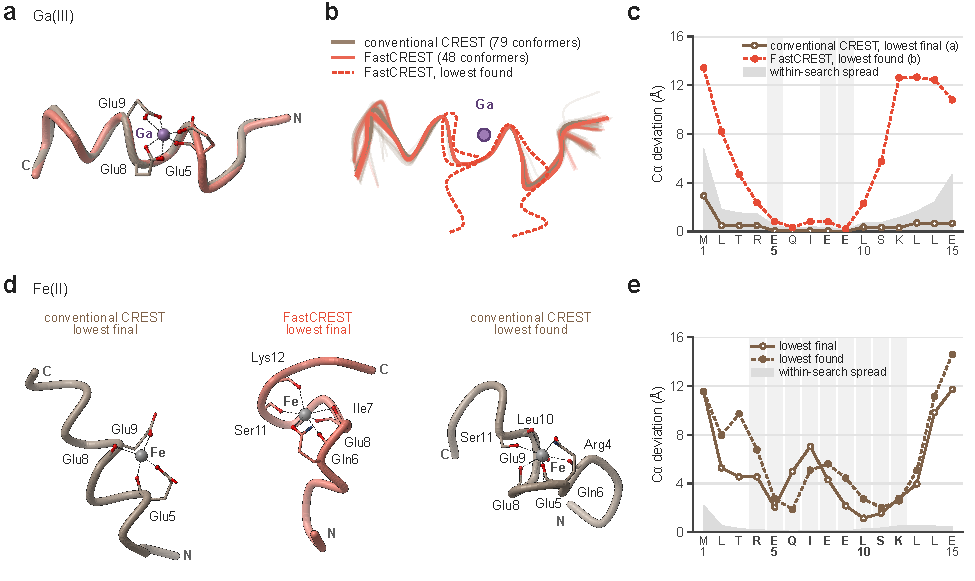
\includegraphics[width=\textwidth]{figures/si_pep023.pdf}
\caption{Lowest structures of the Ga(III) (a--c) and high-spin Fe(II) complexes (d, e) of \mbox{MLTREQIEELSKLLE}, one search
per code; FastCREST red, conventional CREST brown. Every structure is superposed on the metal site of FastCREST's lowest
final conformer: the metal, the backbone of each residue that binds it in any structure compared (Ga: Glu5, Glu8, Glu9;
Fe: Arg4 to Lys12) and the binding side-chain atoms, a carboxylate as its C$\delta$. Tubes trace the C$\alpha$ atoms,
sticks show the binding groups, and dashes join the metal to oxygens within 2.6~\AA{} (Ga) or 2.8~\AA{} (Fe). (a) Lowest
final conformers (FastCREST's 1.1~kcal/mol lower). (b) C$\alpha$ traces of all final conformers, the lowest in bold, and
the lowest structure FastCREST found (dashed; 30.7~kcal/mol lower, dropped at a new cycle). (c) Deviation of each
residue's C$\alpha$ from FastCREST's lowest final conformer, for conventional CREST's (solid) and for the dashed structure
of (b), and the largest deviation of any conformer in (b) from the lowest conformer of its own search (shaded); bold
residues belong to the site. The lowest structure conventional CREST found deviates by at most 0.8~\AA{} and is not
shown. (d) Side by side, in the same orientation and scale: the lowest final conformers of conventional CREST and
FastCREST (85.5~kcal/mol lower), and the lowest structure conventional CREST found (13.7~kcal/mol below FastCREST's
lowest final conformer, dropped at a new cycle). (e) As (c), for the two conventional CREST structures of (d).}
\label{fig:si-pep023}
\end{figure}

\begin{table}[tbp]
\caption{Searches of the Ga(III) and High-Spin Fe(II) Complexes of \mbox{MLTREQIEELSKLLE}. Energies in kcal/mol Relative to
FastCREST's Lowest Final Conformer of Each Complex}
\label{tab:si-pep023}
\small
\setlength{\tabcolsep}{3pt}
\begin{tabular}{@{}L{0.08\textwidth}L{0.215\textwidth}rrrrL{0.245\textwidth}r@{}}
\toprule
complex & structure & time (h) & cycles & conformers & energy & metal donors (CN) & $R_\mathrm{g}$ (\AA) \\
\midrule
Ga(III) & input & & & & & Glu5; Glu8, Glu9 (2 O each); backbone O of Glu5 (6) & 7.49 \\
 & FastCREST & 58.4 & 3 & 48 & 0.0 & same as input (6) & 7.66 \\
 & \quad lowest found\textsuperscript{\emph{a}} & & & & $-30.7$ & same as input (6) & 6.71 \\
 & conventional CREST & 265.8 & 2 & 79 & $+1.1$ & same as input (6) & 7.36 \\
 & \quad lowest found\textsuperscript{\emph{a}} & & & & $-2.4$ & same as input (6) & 7.65 \\
Fe(II) & input & & & & & Glu9; backbone O of Glu5, Glu8 (3) & 7.57 \\
 & FastCREST\textsuperscript{\emph{b}} & 7.3 & 1 & 5 & 0.0 & Gln6 OE1; backbone O of Gln6, Ile7, Glu8, Ser11, Lys12 (6) & 6.57 \\
 & conventional CREST & 242.3 & 4 & 4 & $+85.5$ & Glu5, Glu9; backbone O of Glu5, Glu8 (4) & 7.25 \\
 & \quad lowest found\textsuperscript{\emph{a}} & & & & $-13.7$ & Gln6 OE1, Ser11 OG; backbone O of Arg4, Glu5, Gln6, Glu8, Glu9, Leu10 (8) & 6.45 \\
\bottomrule
\end{tabular}

\smallskip
\begin{minipage}{\textwidth}\raggedright\footnotesize
Time: elapsed time of the main job. Conformers: final ensemble. Energy, donors (within 2.6~\AA{} of Ga or 2.8~\AA{} of
Fe; CN, coordination number) and radius of gyration $R_\mathrm{g}$ of the peptide heavy atoms: lowest final conformer,
or the structure named; a Glu without a count binds one carboxylate oxygen. \textsuperscript{\emph{a}}Lowest structure
the search found; a new cycle dropped it from the final result (Section~\ref{si:cycle}); energy from the search log.
\textsuperscript{\emph{b}}Its lowest final conformer is also the lowest structure it found.
\end{minipage}
\end{table}

\end{document}
